\section{Lenguajes libres de contexto}

\subsection{Gramáticas libres de contexto}

\subsubsection{Gramáticas}

\paragraph{Definición.} Una \textbf{gramática libre de contexto} (CFG) es una tupla:
\alignformula{
    \ca{G} = (V, \Sigma, P, S)
}
\begin{itemize}
    \item $V$ es un conjunto finito de \textbf{variables} o \textbf{no-terminales}.
    \item $\Sigma$ es el alfabeto finito (o \textbf{terminales}) tal que $\Sigma \cap V = \varnothing$.
    \item $P \subseteq V \times(V \cup \Sigma)^*$ es un subconjunto finito de \textbf{reglas} o \textbf{producciones}.
    \item $S \in V$ es la \textbf{variable inicial}.
\end{itemize}

\ejemplo{}{}{
    Considere la gramática $\ca{G} = (V, \Sigma, P, S)$ tal que:
    \begin{itemize}
        \item $V = \{X, Y\}$
        \item $\Sigma = \{a,b\}$
        \item $\{(X, aXb), (X, Y), (Y, \epsilon)\}$
        \item $S = X$
              \begin{align*}
                  \ca{G}: \quad  X & \to aXb      \\
                  X                & \to Y        \\
                  Y                & \to \epsilon
              \end{align*}
    \end{itemize}
}

\paragraph{Notación.} En este texto:
\begin{itemize}
    \item Para las \textbf{variables} en una gramática usaremos letras mayúsculas: $X,Y,Z,A,B,C,\ldots$
    \item Para los \textbf{terminales} en una gramática usaremos letras minúsculas: $a,b,c,\ldots$
    \item Para palabras en $(V \cup \Sigma)^*$ usaremos símbolos: $\alpha, \beta, \gamma, \ldots$
    \item Para una producción $(A,\alpha) \in P$ la escribimos como: $A \to \alpha$
\end{itemize}

\paragraph{Simplificación.} Si tenemos un conjunto de reglas de la forma:
$$
    \begin{array}{lll}
        X & \rightarrow & \alpha_1 \\
        X & \rightarrow & \alpha_2 \\
          & \cdots      &          \\
        X & \rightarrow & \alpha_n
    \end{array}
$$
entonces escribimos estas reglas \textbf{sucintamente} como
$$
    X \to \alpha_1 \mid \alpha_2 \mid \cdots \mid \alpha_n
$$
Recordando que $\alpha_1, \alpha_2, \ldots, \alpha_n \in (V \cup \Sigma)^*$.

\ejemplo{}{}{
    La gramática del ejemplo anterior:
    \begin{align*}
        \ca{G}: \quad  X & \to aXb      \\
        X                & \to Y        \\
        Y                & \to \epsilon
    \end{align*}
    Podemos escribirla en notación \textbf{sucinta} como:
    \begin{align*}
        \ca{G}: \quad X & \to aXb \mid Y \\
        Y               & \to \epsilon
    \end{align*}
}

\paragraph{Producciones.} Sea $\ca{G}$ una CFG. Definimos la relación $\Rightarrow \subseteq(V \cup \Sigma)^* \times(V \cup \Sigma)^*$ de \textbf{producción} tal que:
\alignformula{
    \alpha \cdot X \cdot \beta \Rightarrow \alpha \cdot \gamma \cdot \beta \quad \text { si, y solo si, } \quad(X \rightarrow \gamma) \in P
}
para todo $X \in V$ y $\alpha, \beta, \gamma \in(V \cup \Sigma)^*$. \medbreak

Si $\alpha X \beta \Rightarrow \alpha \gamma \beta$ entonces decimos que:
\begin{itemize}
    \item $\alpha X \beta$ \textbf{produce} $\alpha \gamma \beta$ o
    \item $\alpha \gamma \beta$ \textbf{es producible} desde $\alpha X \beta$.
    \item $\alpha X \beta \Rightarrow \alpha \gamma \beta$ es \textbf{reemplazar} $\gamma$ en $X$ en la palabra $\alpha X \beta$.
\end{itemize}

\paragraph{Derivaciones.} Sea $\ca{G}$ una CFG. Dadas dos palabras $\alpha, \beta \in(V \cup \Sigma)^*$ decimos que $\alpha$ \textbf{deriva} $\beta$:
\alignformula{
    \alpha \overunder{\Rightarrow}{}{*} \beta
}
si existe $\alpha_1, \alpha_2, \ldots, \alpha_n \in(V \cup \Sigma)^*$ tal que: $\alpha \Rightarrow \alpha_1 \Rightarrow \alpha_2 \Rightarrow \ldots \Rightarrow \beta$, con $\overunder{\Rightarrow}{}{*}$ la \textbf{clausura refleja y transitiva} de $\Rightarrow$, esto es:
\begin{enumerate}
    \item $\alpha \overunder{\Rightarrow}{}{*} \alpha$
    \item $\alpha \overunder{\Rightarrow}{}{*} \beta$ si, y sólo si, existe $\gamma$ tal que $\alpha \overunder{\Rightarrow}{}{*} \gamma$ y $\gamma \Rightarrow \beta$.
\end{enumerate}
para todo $\alpha, \beta \in (V \cup \Sigma)^*$. Notemos que $\Rightarrow$ y $\overunder{\Rightarrow}{}{*}$ son relaciones entre palabras en $(V \cup \Sigma)^*$.

\paragraph{Lenguaje.} Sea $\ca{G}$ una CFG. El \textbf{lenguaje} de una gramática $\ca{G}$ se define como:
\alignformula{
    \mathcal{L}(\mathcal{G})=\left\{w \in \Sigma^* \mid S \stackrel{\star}{\Rightarrow} w\right\}
}

$\ca{L}(\ca{G})$ son todas las palabras en $\Sigma^*$ que se pueden derivar desde $S$.

\ejemplo{}{}{
    Sea $\ca{G}$ una CFG tal que:
    \begin{align*}
        \ca{G}: \quad X & \to aXb \mid Y \\
        Y               & \to \epsilon
    \end{align*}
    \begin{itemize}
        \item Como $X \overunder{\Rightarrow}{}{*} aaabbb$, entonces $aaabbb \in \ca{L}(\ca{G})$.
        \item En general, uno puede demostrar por \textbf{inducción} que:
              $$
                  \mathcal{L}(\mathcal{G})=\left\{a^n b^n \mid n \geq 0\right\}
              $$
    \end{itemize}
}

\paragraph{Lenguaje libre de contexto.} Diremos que $L \subseteq \Sigma^*$ es un \textbf{lenguaje libre de contexto} si, y sólo si, existe una gramática libre de contexto $\ca{G}$ tal que:
\alignformula{
    L = \ca{L}(\ca{G})
}

\ejemplo{}{}{
    Los siguientes son lenguajes libres de contexto:
    \begin{itemize}
        \item $L=\left\{a^n b^n \mid n \geq 0\right\}$
        \item $\text{Par}=\left\{w \in\{a, b\}^* \mid w \text { tiene largo par }\right\}$
        \item $\text{Pal}=\left\{w \in\{a, b\}^* \mid w=w^{\mathrm{rev}}\right\}$
    \end{itemize}
}

\subsubsection{Árboles y derivaciones}

\paragraph{Definición.} El conjunto de \textbf{árboles ordenados y etiquetados} (o solo árboles) sobre etiquetas $\Sigma$ y $V$, se define recursivamente como:
\begin{itemize}
    \item $t:=a$ es un árbol para todo $a \in \Sigma$.
    \item si $t_1,\ldots, t_k$ son árboles, entonces $t:= X(t_1, \ldots, t_k)$ es un árbol para todo $X \in V$.
\end{itemize}

Para un árbol $t = X(t_1,\ldots,t_k)$ cualquiera se define:
\begin{itemize}
    \item $\texttt{raiz}(t)=X$
    \item $\texttt{hijos}(t)= t_1,\ldots,t_k$
\end{itemize}

Si $t = a$, entonces decimos que $t$ es una \textbf{hoja}, $\texttt{raiz}(t) = a$ y $\texttt{hijos}(t) = \epsilon$.

\paragraph{Definición.} Fije una CFG $\ca{G} = (V, \Sigma, P, S)$. Se define el conjunto de \textbf{árboles de derivación} recursivamente como:
\begin{itemize}
    \item Si $a \in \Sigma$, entonces $t = a$ es un árbol de derivación.
    \item Si $X \to X_1 \ldots X_k \in P$ y $t_1,\ldots,t_k$ son árboles de derivación con $\texttt{raiz}(t) = X_i$ para todo $i \leq k$, entonces $t = X(t_1,\ldots,t_k)$ es un árbol de derivación.
\end{itemize}

Decimos que $t$ es un \textbf{árbol de derivación de} $\ca{G}$ si:
\begin{enumerate}
    \item $t$ es un árbol de derivación y
    \item $\texttt{raiz}(t) = S$.
\end{enumerate}
Los árboles de derivación son todos los árboles que parten desde $S$.

\ejemplo{}{}{
    Sea $\ca{G}$ una CFG tal que:
    $$
        G: \quad E \; \to \; E + E \mid E * E \mid n
    $$
    Algunos árboles de derivación para $\ca{G}$ son:
    \img{img/cap4/ejemplo5.png}{0.45}
}

\paragraph{Definición.} Sea $\ca{G}$ una CFG y $w \in \Sigma^*$. Se define la función $\texttt{yield}$ sobre árboles, recursivamente como:
\begin{itemize}
    \item Si $t = a \in \Sigma$, entonces $\texttt{yield}(t) = a$.
    \item Si $t$ no es una hoja y $\texttt{hijos}(t) = t_1 t_2 \ldots t_k$, entonces:
          $$
              \texttt{yield}(t) =\texttt{yield}(t_1) \cdot \texttt{yield}(t_2) \cdot \ldots \cdot \texttt{yield}(t_k)
          $$
\end{itemize}

Decimos que $t$ es un \textbf{árbol de derivación de} $\ca{G}$ \textbf{para} $w$ si:
\begin{enumerate}
    \item $t$ es un árbol de derivación de $\ca{G}$ y
    \item $\texttt{yield}(t) = w$
\end{enumerate}
Lo anterior significa que las hojas de $t$ forman la palabra $w$.

\paragraph{Proposición.} Sea $\ca{G} = (V, \Sigma, P, S)$ una CFG y $w \in \Sigma^*$. Tenemos que:
$$
    w \in \mathcal{L}(\mathcal{G}) \quad \text { si, y solo si,} \quad \text{existe un árbol de derivación de } \mathcal{G} \text { para } w.
$$
Un árbol de derivación es la \textbf{representación grática} de una derivación.

\ejemplo{}{}{
    \vspace{-10pt}
    \img{img/cap4/ejemplo6.png}{0.4}
}

\paragraph{Definición.} Sea $\ca{G} = (V, \Sigma, P, S)$ una CFG.
\begin{itemize}
    \item Definimos la \textbf{derivación por la izquierda} $\underset{\mathrm{lm}}{\Rightarrow} \; \subseteq(V \cup \Sigma)^* \times(V \cup \Sigma)^*$:
          \alignformula{
              w \cdot X \cdot \beta \underset{\mathrm{lm}}{\Rightarrow} w \cdot \gamma \cdot \beta \quad \text { si, y solo si, } \quad X \rightarrow \gamma \in P
          }
          para todo $X \in V$, $w \in \Sigma^*$ y $\beta,\gamma \in (V \cup \Sigma)^*$.

    \item Definimos la \textbf{derivación por la derecha} $\underset{\mathrm{rm}}{\Rightarrow} \; \subseteq(V \cup \Sigma)^* \times(V \cup \Sigma)^*$:
          \alignformula{
              \alpha \cdot X \cdot w \underset{\mathrm{rm}}{\Rightarrow} \alpha \cdot \gamma \cdot w \quad \text { si, y solo si, } \quad X \rightarrow \gamma \in P
          }
          para todo $X \in V$, $w \in \Sigma^*$ y $\alpha,\gamma \in (V\cup \Sigma)^*$.
\end{itemize}

Se define $\overunder{\Rightarrow}{\mathrm{lm}}{*}$ y $\overunder{\Rightarrow}{\mathrm{rm}}{*}$ como la \textbf{clausura refleja y transitiva} de $\overunder{\Rightarrow}{\mathrm{lm}}{}$ y $\overunder{\Rightarrow}{\mathrm{rm}}{}$, respectivamente.  \medbreak

$\overunder{\Rightarrow}{\mathrm{lm}}{}$ y $\overunder{\Rightarrow}{\mathrm{rm}}{}$ solo reemplaza \textbf{a la izquierda} (leftmost) y \textbf{derecha} (rightmost).

\ejemplo{}{}{
    \vspace{-10pt}
    \img{img/cap4/ejemplo7.png}{0.4}
}

\paragraph{Proposicion.} Por cada árbol de derivación, existe una \textbf{única} derivación por la izquierda y una \textbf{única} derivación por la derecha. \medbreak

Por lo tanto, desde ahora podemos hablar de \textbf{árbol de derivación y derivación (izquierda o derecha)} indistintamente.

\subsubsection{Lenguajes regulares vs libres de contexto}

\paragraph{Proposición.} Para todo lenguaje regular $L$, existe una gramática libre de contexto $\ca{G}_\ca{A}$:
\alignformula{
    L = \ca{L}(\ca{G}_\ca{A})
}

\paragraph{Idea demostración.} Dado un autómata finito determinista $\ca{A} = (Q, \Sigma, \delta, q_0, F)$, ¿cómo construimos una gramática libre de contexto? \medbreak

Defina la gramática $\ca{G}_\ca{A} = (Q, \Sigma, P_\ca{A}, q_0)$ tal que:
\begin{itemize}
    \item si $\delta(p,a) = q$, entonces $p \to aq \in P\ca{A}$
    \item si $p \in F$, entonces $p \to \epsilon \in P_\ca{A}$
\end{itemize}

Queda como ejercicio propuesto al lector demostrar que $\ca{L}(\ca{A}) = \ca{L}(\ca{G}_\ca{A})$

\subsection{Simplificación de gramáticas}

¿Cómo podemos simplificar la siguiente gramática?
\begin{align*}
    G: \quad S \  & \to \ aAa \mid aBD \mid aBH \\
    A \           & \to \ B \mid D              \\
    B \           & \to \ aBa \mid b            \\
    C \           & \to \ aCC \mid bC           \\
    D \           & \to \ aDCa \mid CFa         \\
    F \           & \to \ aFDa \mid aab         \\
    H \           & \to \ \epsilon
\end{align*}
\begin{enumerate}
    \item Dada una variable $X$, ¿es $X$ \textbf{útil} para producir palabras?
    \item Dada una producción $p:X \to \gamma$, ¿es $p$ \textbf{útil} para producir palabras?
\end{enumerate}

\subsubsection{Eliminación de variables inútiles}

\paragraph{Definición.} Sea $\ca{G} = (V,\Sigma,P,S)$ una CFG. Diremos que una variable $X \in V$ es \textbf{útil} si existe una derivación:
\alignformula{
    S \stackrel{\star}{\Rightarrow} \alpha X \beta \stackrel{\star}{\Rightarrow} w
}
Al contrario, diremos que una variable $X$ es \textbf{inútil} si NO es útil.

\paragraph{Definición.} Para una variable $X \in V$:
\begin{enumerate}
    \item Decimos que $X$ es \textbf{alcanzable} si existe una derivación:
          \alignformula{
              S \stackrel{\star}{\Rightarrow} \alpha X \beta
          }
    \item Decimos que $X$ es \textbf{generadora} si existe una derivación:
          \alignformula{
              X \stackrel{\star}{\Rightarrow} w
          }
\end{enumerate}

\paragraph{Propiedad.} Para toda variable $X \in V - \{S\}$:
\alignformula{
    \text{existe una producción } Y \to \alpha X \beta \in P \text{ tal que } Y \in V \text{ es alcanzable} \quad \Leftrightarrow \quad X \text{ es alcanzable.}
}
La demostración de esta propiedad queda como ejercicio propuesto al lector. \medbreak

Un algoritmo para determinar si una variable es alcanzable:
\begin{algorithm}[hbt!]
    \setstretch{1.25}
    \DontPrintSemicolon
    \SetKwFunction{Falcanzables}{alcanzables}
    \SetKwProg{Fn}{Function}{:}{}
    \SetKwInOut{Input}{input}\SetKwInOut{Output}{output}
    \SetKw{Let}{let}
    \SetKw{Take}{take}
    \Input{Gramática $\ca{G}=(V,\Sigma,P,S)$}
    \Output{Conjunto $C$ de variables alcanzables}
    \Fn{\Falcanzables{$\ca{G}$}}{
        \Let $C_0 := \{S\}$

        \Let $C := \varnothing$

        \While{$C_0 \neq \varnothing$}{
            \Take $Y \in C_0$

            $C_0 := C_0 - \{Y\}$

            $C := C \cup \{Y\}$

            \ForEach{$X \in V - C$ \textit{tal que existe una regla} $\Big(Y \to \alpha X \beta\Big) \in P$}{
                $C_0 := C_0 \cup \{X\}$
            }
        }

        \Return $C$
    }
\end{algorithm}

\paragraph{Propiedad.} Para toda variable $X \in V$:
\alignformula{
    \text{existe una regla } X \to \alpha \text{ tal que todas las variables en } \alpha \text{ son generadoras} \quad \Leftrightarrow \quad X \text{ es generadora.}
}

La demostración de esta propiedad queda como ejercicio propuesto al lector. \medbreak

Un algoritmo para determinar si una variable es generadora:

\begin{algorithm}[hbt!]
    \setstretch{1.25}
    \DontPrintSemicolon
    \SetKwFunction{Falcanzables}{alcanzables}
    \SetKwProg{Fn}{Function}{:}{}
    \SetKwInOut{Input}{input}\SetKwInOut{Output}{output}
    \SetKw{Let}{let}
    \SetKw{Take}{take}
    \Input{Gramática $\ca{G}=(V,\Sigma,P,S)$}
    \Output{Conjunto $G$ de variables generadoras}
    \Fn{\Falcanzables{$\ca{G}$}}{
        \Let $G_0 := \{X \in V \mid (X \to w) \in P\}$

        \Let $G := \varnothing$

        \While{$G_0 \neq G$}{
            $G := G_0$

            \ForEach{$(X \to \alpha) \in P$}{
                \If{\textit{todas las variables en} $\alpha$ \textit{estan en} $G$}{
                    $G_0 := G_0 \cup \{X\}$
                }
            }
        }

        \Return $G$
    }
\end{algorithm}

\teorema{}{}{
    Sea $G = (V, \Sigma, P, S)$ una CFG. Sea $\ca{G}''$ una gramática creada a partir de $\ca{G}$ después de:
    \begin{itemize}
        \item eliminar todas las variables y reglas NO generadoras.
        \item eliminar todas las variables y reglas NO alcanzables.
    \end{itemize}
    Entonces, $\ca{L}(\ca{G}'') = \ca{L}(\ca{G})$ y $\ca{G}''$ no contiene variables inútiles.
}

\textbf{Nota:} Debemos respetar el orden para eliminar variables generadoras y luego las alcanzables. De hacerlo al revés, la gramática resultante puede no definir el mismo lenguaje que la inicial.

\paragraph{Demostración teorema 18.} Sea $\ca{G} = (V, \Sigma, P, S)$ una CFG. \medbreak

Sea $\ca{G}' = (V', \Sigma, P', S)$ al eliminar las variables \textbf{no generadoras} de $\ca{G}$:
$$
    \begin{aligned}
        V^{\prime} & =\{X \in V \mid \exists w.\ X \underset{\mathcal{G}}{\stackrel{\star}{\Rightarrow}} w\}                                 \\
        P^{\prime} & =\left\{X \rightarrow \alpha \in P \mid X \in V^{\prime} \wedge \alpha \in\left(V^{\prime} \cup \Sigma\right)^*\right\}
    \end{aligned}
$$

Sea $\ca{G}'' = (V'', \Sigma, P'', S)$ al eliminar las variables \textbf{no alcanzables} de $\ca{G}'$:
$$
    \begin{aligned}
        V^{\prime \prime} & =\left\{X \in V^{\prime} \mid \exists \alpha, \beta.\ S \underset{\mathcal{G}^{\prime}}{\stackrel{\star}{\Rightarrow}} \alpha X \beta\right\}  \\
        P^{\prime \prime} & =\left\{X \rightarrow \alpha \in P^{\prime} \mid X \in V^{\prime \prime} \wedge \alpha \in\left(V^{\prime \prime} \cup \Sigma\right)^*\right\}
    \end{aligned}
$$

Considere las siguientes propiedades de $\ca{G}$, $\ca{G}'$ y $\ca{G}''$:
\begin{enumerate}
    \item Para todo $\alpha \in (V \cup \Sigma)*$, si $\alpha \overunder{\Rightarrow}{\ca{G}}{*} w$ entonces $\alpha \overunder{\Rightarrow}{\ca{G}'}{*} w$.

    \item Para todo $\alpha \in (V' \cup \Sigma)*$, si $S \overunder{\Rightarrow}{\ca{G}'}{*} \alpha$ entonces $S \overunder{\Rightarrow}{\ca{G}''}{*} \alpha$

    \item Para todo $\alpha \in (V'' \cup \Sigma)*$, si $\alpha \overunder{\Rightarrow}{\ca{G}'}{*} w$ entonces $\alpha \overunder{\Rightarrow}{\ca{G}''}{*} w$.
\end{enumerate}

La demostración de estas propiedades queda como ejercicio propuesto al lector. \bigbreak

\textit{Demostración $\mathcal{L}\left(\mathcal{G}^{\prime \prime}\right) \subseteq \mathcal{L}(\mathcal{G})$.} Como $V'' \subseteq V$ y $P'' \subseteq P$, entonces es trivial que $\mathcal{L}\left(\mathcal{G}^{\prime \prime}\right) \subseteq \mathcal{L}(\mathcal{G})$. \bigbreak

\textit{Demostración $\mathcal{L}(\mathcal{G}) \subseteq \mathcal{L}\left(\mathcal{G}^{\prime \prime}\right)$.} Sea $w \in \ca{L}(\ca{G})$ tal que $S \overunder{\Rightarrow}{\ca{G}}{*} w$.
\begin{itemize}
    \item Por la propiedad 1, tenemos que $S \overunder{\Rightarrow}{\ca{G}'}{*} w$.
    \item Por la propiedad 2, tenemos que $S \overunder{\Rightarrow}{\ca{G}''}{*} w$.
\end{itemize}

Por lo tanto $w \in \ca{L}(\ca{G}'')$ y concluimos que $\mathcal{L}\left(\mathcal{G}^{\prime \prime}\right) \subseteq \mathcal{L}(\mathcal{G})$. \bigbreak

\textit{Demostración variables útiles.} Queremos mostrar que para todo $X \in V''$, $X$ es \textbf{útil} en $\ca{G}''$. \bigbreak

Como $X \in V''$, entonces $S \overunder{\Rightarrow}{\ca{G}'}{*} \alpha X \beta$ para algún $\alpha, \beta \in\left(V^{\prime} \cup \Sigma\right)^*$. \medbreak

Por la propiedad 2, se tiene que: $S \overunder{\Rightarrow}{\ca{G}''}{*} \alpha X \beta$ y $\alpha, \beta \in\left(V^{\prime \prime} \cup \Sigma\right)^*$. \medbreak

Como $X \in V'$ y $\alpha,\beta \in (V' \cup \Sigma)^*$, entonces existen $u, v, w$ tal que:
$$
    \alpha \overunder{\Rightarrow}{\ca{G}}{*} u, \quad X \overunder{\Rightarrow}{\ca{G}}{*} v, \quad \beta \overunder{\Rightarrow}{\ca{G}}{*} w
$$

Por la propiedad 1, se tiene que: $\alpha \overunder{\Rightarrow}{\ca{G}'}{*} u, \quad X \overunder{\Rightarrow}{\ca{G}'}{*} v, \quad \beta \overunder{\Rightarrow}{\ca{G}'}{*} w$. \medbreak

Por la propiedad 3, se tiene que: $\alpha \overunder{\Rightarrow}{\ca{G}''}{*} u, \quad X \overunder{\Rightarrow}{\ca{G}''}{*} v, \quad \beta \overunder{\Rightarrow}{\ca{G}''}{*} w$. \medbreak

Juntando todo, $S \overunder{\Rightarrow}{\ca{G}''}{*} \alpha X \beta \overunder{\Rightarrow}{\ca{G}''}{*} uvw$ y por tanto $X$ es útil en $\ca{G}''$. \hfill $\blacksquare$

\subsubsection{Eliminación de producciones inútiles}

\paragraph{Definición.} Sea $\ca{G}$ una CFG. Decimos que:
\begin{itemize}
    \item Una producción de la forma $X \to \epsilon$ es \textbf{en vacío}.
    \item Una producción de la forma $X \to Y$ es \textbf{unitaria}.
\end{itemize}

Deseamos eliminar este tipo de producciones para simplificar nuestras gramáticas, sin embargo, debemos tener cuidado con algunos detalles.

\paragraph{Proposición.} Si $\epsilon \in \ca{L}(\ca{G})$, entonces NO se pueden borrar las producciones en vacío sin alterar el lenguaje $\ca{G}$. \medbreak

Así que, desde ahora, supondremos que $\epsilon \notin \ca{L}(\ca{G})$.

\paragraph{Definición.} Sea $\ca{G} = (V, \Sigma, P, S)$ una CFG tal que $\epsilon \notin \ca{L}(\ca{G})$. Definimos a $P^*$ como el \textbf{menor conjunto de producciones} que contiene a $P$ y \textbf{cerrado bajo} las siguientes reglas:
\begin{enumerate}
    \item Si $X \to Y \in P^*$ y $Y \to \gamma \in P^*$, entonces $X \to \gamma \in P^*$.
    \item Si $X \to \epsilon \in P^*$ y $Z \to \alpha X \beta \in P^*$, entonces $Z \to \alpha \beta \in P^*$.
\end{enumerate}
Definimos $\ca{G}^* = (V, \Sigma, P^*, S)$. Entonces:
\begin{itemize}
    \item $P^*$ es finito y
    \item $\ca{L}(\ca{G}^*) = \ca{L}(\ca{G})$.
\end{itemize}

Ahora, para cualquier palabra $w \in \ca{L}(\ca{G}^*)$, sea $\ca{T}$ un árbol de derivación de $w$ en $\ca{G}^*$ de \textbf{tamaño mínimo}. Definimos las siguientes propiedades:
\begin{enumerate}
    \item El árbol de derivación $\ca{T}$ NO usa una \textbf{producción unitaria}.
    \item El árbol de derivación $\ca{T}$ NO usa una producción \textbf{en vacío}.
\end{enumerate}

La demostración de estas propiedades se hace por contradicción: se supone que $\ca{T}$ usa una producción unitaria o en vacío y se comprueba que si ocurre esto entonces $\ca{T}$ no tiene tamaño mínimo. \bigbreak

Por la propiedad 1 y 2, tenemos que \textit{para todo $w \in \ca{L}(\ca{G}^*)$, existe una derivación de $w$ en $\ca{G}$ que NO usa producciones \textbf{en vacío} ni producciones \textbf{unitarias}}. Por lo tanto, podemos eliminar las producciones en vacío y unitarias de $\ca{G}^*$.

\teorema{}{}{
    Para toda CFG $\ca{G}$ tal que $\epsilon \notin \ca{L}(\ca{G})$, sea:
    \begin{itemize}
        \item $\ca{G}^*$ la clausura de producciones unitarias y en vacío.
        \item $\hat{\ca{G}}$ el resultado de remover toda producción unitaria o en vacío de $\ca{G}^*$.
    \end{itemize}
    Entonces, $\ca{L}(\hat{\ca{G}}) = \ca{L}(\ca{G})$ y $\hat{\ca{G}}$ no tiene producciones unitarias o en vacío.
}

Resumiendo, para eliminar las producciones en vacío y unitarias de $\ca{G}$:
\begin{itemize}
    \item construimos $\ca{G}^*$ haciendo la \textbf{clausura} de producciones unitarias y en vacío,
    \item construimos $\hat{\ca{G}}$ \textbf{removiendo} todas las producciones unitarias o en vacío de $\ca{G}^*$.
\end{itemize}
Por el resultado anterior sabemos que $\ca{L}(\hat{\ca{G}}) = \ca{L}(\ca{G})$. Es importante mencionar que es posible que $\hat{\ca{G}}$ contenga símbolos inútiles.

\subsection{Forma normal de Chomsky}

\paragraph{Definición.} Una gramática $\ca{G}$ esta en \textbf{forma normal de Chomsky} (CNF) si todas sus reglas son de la forma:
\begin{itemize}
    \item $X \to YZ$
    \item $X \to a$
\end{itemize}
\ejemplo{}{}{
    La siguiente gramática está en CNF:
    \begin{align*}
        S \  & \to \ AB \mid AC \mid SS \\
        C \  & \to \ SB                 \\
        A \  & \to a                    \\
        B \  & \to b
    \end{align*}
}
Toda gramática se puede convertir en CNF. Para facilitar el proceso, considere $\ca{G} = (V, \Sigma, P, S)$ una CFG tal que $\epsilon \notin \ca{L}(\ca{G})$.
\begin{itemize}
    \item Primero, suponga que $\ca{G}$ no contiene reglas en vacío o unitarias.
    \item Por lo tanto, todas las reglas en $\ca{G}$ son de la forma:
          \begin{itemize}
              \item $X \to \gamma \quad $ para $|\gamma| \geq 2$
              \item $X \to a$
          \end{itemize}
\end{itemize}

Los pasos para convertir $\ca{G}$ en CNF son:
\begin{enumerate}
    \item Convertir todas las reglas a la forma:
          \begin{itemize}
              \item $X \to Y_1 Y_2 \ldots Y_k$ para $k \geq 2$
              \item $X \to a$
          \end{itemize}

    \item Convertir todas las reglas a la forma:
          \begin{itemize}
              \item $X \to YZ$
              \item $X \to a$
          \end{itemize}
\end{enumerate}

Para realizar el paso 1:
\begin{itemize}
    \item Para cada $a \in \Sigma$, agregamos una nueva variable $X_a$ y una regla $X_a \to a$.
    \item Reemplazamos todas las ocurrencias antiguas de $a$ por $X_a$.
\end{itemize}

\ejemplo{}{}{
    Considere la gramática $S \to aSb \mid ab$, entonces, hacer el paso 1 termina en:
    \begin{align*}
        S \  & \to \ ASB \mid AB \\
        A \  & \to \ a           \\
        B \  & \to \ b
    \end{align*}
}

\paragraph{Correctitud.} Si $\ca{G}'$ es la gramática resultante del paso 1, entonces se cumple que $\ca{L}(\ca{G}') = \ca{L}(\ca{G})$. \bigbreak

Para realizar el paso 2, tomamos cada regla $p: X \to Y_1 Y_2 \ldots Y_k$ con $k \geq 3$ y:
\begin{itemize}
    \item Agregamos una \textbf{nueva} variable $Z$.
    \item Reemplazamos la regla $p$ por \textbf{dos reglas}:
          $$
              X \to Y_1 Z \quad \text{y} \quad Z \to Y_2 \ldots Y_k
          $$
\end{itemize}
Repetimos este paso hasta llegar a la forma normal de Chosmky.

\ejemplo{}{}{
    El resultado del paso 1 anterior es:
    \begin{align*}
        S \  & \to \ ASB \mid AB \\
        A \  & \to \ a           \\
        B \  & \to \ b
    \end{align*}
    Al realizar el paso 2, la gramática queda de la forma:
    \begin{align*}
        S \  & \to \ AZ \mid AB \\
        Z \  & \to SB           \\
        A \  & \to \ a          \\
        B \  & \to \ b
    \end{align*}
}

\paragraph{Correctitud.} Si $\ca{G}''$ es la gramática resultante del paso 2, entonces se cumple que $\ca{L}(\ca{G}'') = \ca{L}(\ca{G}')$.

\teorema{}{}{
    Sea $\ca{G} = (V, \Sigma, P, S)$ una CFG tal que $\epsilon \notin \ca{L}(\ca{G})$. Existe una gramática $\ca{G}'$ en forma normal de Chomsky tal que:
    $$
        \ca{L}(\ca{G}') = \ca{L}(\ca{G})
    $$
}

Si $\ca{G}'$ no tiene reglas unitarias ni en vacío, entonces $\ca{G}'$ es de \textbf{tamaño polinomial} con respecto a $\ca{G}$.

\subsection{Lema de bombeo para lenguajes libres de contexto}

Similarmente para los lenguajes regulares, existe un lema de bombeo para lenguajes libres de contexto. \bigbreak

Sea $L\subseteq \Sigma^*$. Si $L$ es \textbf{libre de contexto}, entonces:
\alignformula{
    (\text{LB}^\text{CFL}) \quad &\text{existe un } N > 0 \text{ tal que}\\
    &\text{para toda palabra } z \in L \text{ con } |z| \geq N \\
    &\text{existe una descomposición } z = uvwxy \\
    &\hphantom{aaaaa} \text{con } vx \neq \epsilon \text{ y } |vwx| \leq N \text{ tal que}\\
    &\text{para todo } i \geq 0,\; u \cdot v^i \cdot w \cdot x^i \cdot y \in L
}

Análogamente, para demostrar que un lenguaje $L$ NO es libre de contexto, usamos el contrapositivo del lema. \bigbreak

Sea $L \subseteq \Sigma^*$. Si:
\alignformula{
    (\neg\text{LB}^\text{CFL}) \quad &\text{para todo } N > 0 \text{ tal que}\\
    &\text{existe una palabra } z \in L \text{ con } |z| \geq N \\
    &\text{para toda descomposición } z = uvwxy \\
    &\hphantom{aaaaa} \text{con } vx \neq \epsilon \text{ y } |vwx| \leq N \text{ tal que}\\
    &\text{existe } i \geq 0,\; u \cdot v^i \cdot w \cdot x^i \cdot y \notin L\\
    &\hphantom{aaaaa} \text{entonces } L \text{ NO es libre de contexto}.
}
\paragraph{Jugando contra un demonio.} El lema de bombeo puede verse como el siguiente ``juego'':
\img{img/cap4/demonio.png}{0.3}

\ejemplo{}{}{
    Considere el lenguaje $L = \{ a^{n^2} \mid n > 0\}$
    \img{img/cap4/ejemplo11.png}{0.25}

    Ganamos ya que al bombear con $i = 2$ ya no se cumple que $j + k + l + m + n = N^2$ (se rompe el equilibrio), y entonces $z \notin L$.
}

\newpage

\ejemplo{}{}{
    Considere el lenguaje $L = \{a^n b^n c^n \mid n > 0\}$.
    \img{img/cap4/ejemplo12.png}{0.25}

    Ganamos el juego, ya que, como $uvwxy = a^N b^N c^N$ con $vx \neq \epsilon$ y $|vwx| \leq N$, entonces
    $$
        vwx \in \ca{L}(a^* b^*) \quad \text{o} \quad vwx \in \ca{L}(b^* c^*)
    $$
    \begin{itemize}
        \item Si $vwx \in \ca{L}(a^+ b^+)$, entonces:
              \begin{itemize}
                  \item $|u v^2 w x^2 y|_{a,b} > 2N$
                  \item $|u v^2 w x^2 y|_{c} = N$
              \end{itemize}
              Por lo tanto, $z' \notin L$.

        \item Si $vwx \in \ca{L}(b^+ c^+)$, entonces:
              \begin{itemize}
                  \item $|u v^2 w x^2 y|_{b,c} > 2N$
                  \item $|u v^2 w x^2 y|_{a} = N$
              \end{itemize}
              Por lo tanto, $z' \notin L$.
    \end{itemize}
    En ambos casos, $uv^2 w x^2 y \notin L$, y por tanto $L$ no es CFG.
}

\paragraph{Lema versión juego.} \textit{``Dado un lenguaje $L \subseteq \Sigma^*$, si \textbf{UNO} tiene una estrategia ganadora en el juego $(\neg\text{LB}^\text{CFL})$ para toda estrategia posible del demonio, entonces $L$ \textbf{NO} es libre de contexto''.}

\paragraph{Consecuencias.} Podemos establecer la siguiente proposición en base al lema de bombeo:
\begin{itemize}
    \item Para todos lenguajes libres de contexto $L_1$ y $L_2$, se cumple que $L_1 \cup L_2$ es un lenguaje libre de contexto.
    \item Existen lenguajes libres de contexto $L$, $L_1$ y $L_2$ tales que:
          \begin{itemize}
              \item $L_1 \cap L_2$ \textbf{NO} es un lenguaje libre de contexto.
              \item $L^C$ \textbf{NO} es un lenguaje libre de contexto.
          \end{itemize}
\end{itemize}

Para demostrar que la intersección no es libre de contexto, basta con un contraejemplo. Tomemos $L_1 = \{a^n b^n c^m \mid n\geq 0, m \geq 0\}$ y $L_2 = \{a^m b^n c^n \mid n \geq 0, m \geq 0\}$, al hacer su intersección, obtendremos el lenguaje $L = \{a^n b^n c^n \mid n \geq 0\}$, que ya vimos que no es libre de contexto. \medbreak

Queda como ejercicio propuesto para el lector demostrar que $L^C$ no es libre de contexto.

\subsection{Algoritmo CKY}

Dado un lenguaje libre de contexto $L$ y una palabra $w$, ¿cómo verificamos si $w \in L$?
\begin{itemize}
    \item Convertimos $\ca{G}$ en forma normal de Chomsky.
    \item Probamos todas las derivaciones de altura a lo más $|w| + 1$.
    \item Si encontramos una derivación retornamos $\texttt{TRUE}$.
\end{itemize}

Los pasos anteriores se conoce como el algoritmo CKY, inventado por John Cocke, Tadao Kasami y Daniel Younger. Es un algoritmo que usa \textbf{programación dinámica}, y es \textbf{cúbico} en $|w|$ y \textbf{lineal} en $|\ca{G}|$:
\alignformula{
    \text{Tiempo:}\; \ca{O}(|w|^3 \cdot |\ca{G}|)
}
Por simplicidad, asumiremos que las gramáticas que recibe el algoritmo están en \textbf{Forma Normal de Chomsky} (CNF).

\paragraph{Tabla del algoritmo CKY.} Para una palabra $w = a_1 a_2 \ldots a_n$ y una gramática $\ca{G} = (V, \Sigma, P, S)$ construimos la \textbf{tabla CKY}:

\img{img/cap4/cky1.png}{0.35}

Para todo $1 \leq 1 \leq j \leq n$ se define:
$$
    C_{i\, j} = \{X \in V \mid X \overunder{\Rightarrow}{\ca{G}}{*} a_i \ldots a_j\}
$$

\begin{multicols}{2}

    \paragraph{Paso 0 (inicial).} Para cada $i$, construimos el conjunto $C_{ii} \subseteq V$ tal que:
    $$
        C_{i\,i} = \{X \in V \mid X \to a_i \in P\}
    $$
    \img{img/cap4/cky2.png}{0.3}

    \paragraph{Paso 1.} Para cada $i$, construimos el conjunto $C_{i\, i +1} \subseteq V$ tal que:
    \begin{align*}
        C_{i\, i+1} =\; & \{X \in V \mid X \to YZ \in P \text{ para algún } \\
                        & Y \in C_{ii} \wedge Z \in C_{i+1 i+1}\}
    \end{align*}

    \img{img/cap4/cky3.png}{0.3}
\end{multicols}

\paragraph{Paso $k$ $(k > 0)$.} Para cada $i$, construimos el conjunto $C_{i\, i+k} \subseteq V$ tal que:
$$
    C_{i\, i+k} = \{ X \in V \mid \exists j \in [i,i+k].\ X \to YZ \in P \text{ para algún } Y \in C_{i\, j} \wedge Z \in C_{j+i \, i+k}\}
$$
\begin{figure}[H]
    \centering
    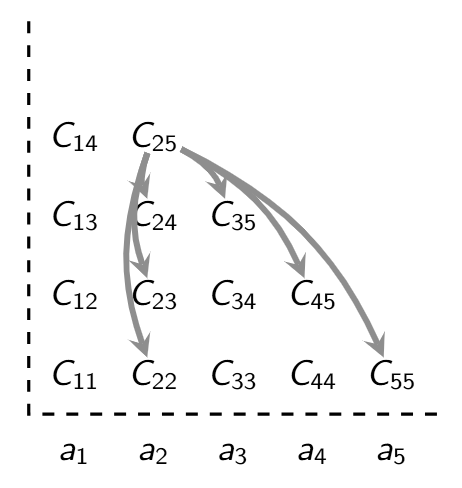
\includegraphics[scale=0.35]{img/cap4/cky4.png}
    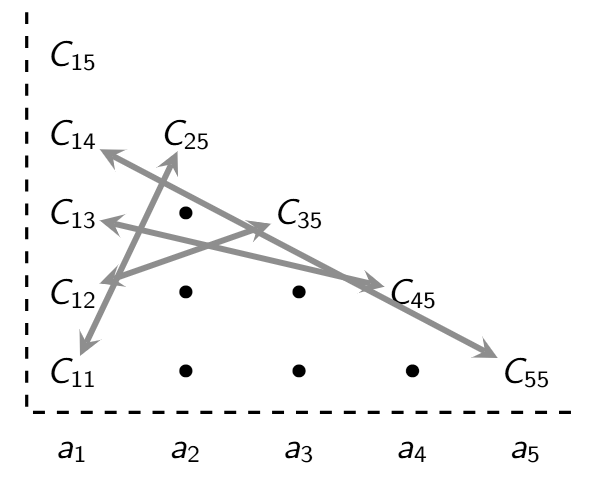
\includegraphics[scale=0.35]{img/cap4/cky5.png}
\end{figure}

\ejemplo{}{}{
    Considere la palabra $bbaba$ y la gramática:
    \img{img/cap4/ejemplo13.png}{0.6}

    Considere la palabra $abba$ y la gramática:
    \img{img/cap4/ejemplo13_1.png}{0.6}
}
\newpage
\paragraph{Algoritmo CKY.} A continuación se muestra el pseudo-código del algoritmo:

\begin{algorithm}[hbt!]
    % \caption*{An algorithm with caption}\label{alg:two}
    \setstretch{1.5}
    \DontPrintSemicolon
    \SetKwFunction{FAlgoritmoCKY}{AlgoritmoCKY}
    \SetKwProg{Fn}{Function}{:}{}
    \SetKwInOut{Input}{input}\SetKwInOut{Output}{output}
    \SetKw{Let}{let}
    \SetKw{Check}{check}
    \Input{Una gramática $\ca{G}=(V,\Sigma,P,S)$ y una palabra $w = a_1 a_2 \ldots a_n$}
    \Output{$\texttt{TRUE}$ si, y sólo si, $w \in \ca{L}(\ca{G})$}
    \Fn{\FAlgoritmoCKY{$\ca{G},w$}}{
        \For{$i = 1$ \KwTo $n$}{
            \Let $C_{i\, i} = \varnothing$

            \For{$X \to C \in P$}{
                \If{$c = a_i$}{\Let $C_{i\, i} = C_{i\, i} \cup \{X\}$}
            }
        }

        \For{$k=1$ \KwTo $n - 1$}{
            \For{$i=1$ \KwTo $n-k$}{
                \Let $C_{i\, i+k} = \varnothing$

                \For{$j = i$ \KwTo $i+k-1$}{
                    \For{$X \to YZ \in P$}{
                        \If{$Y \in C_{i\, j} \wedge Z \in C_{j+1\, i+k}$}{
                            \Let $C_{i\, i+k} = C_{i\, i+k} \cup \{X\}$
                        }
                    }
                }
            }
        }

        \Return \Check $S \in C_{1\, n}$
    }
\end{algorithm}

\paragraph{Análisis algoritmo CKY.} En su correctitud, para toda gramática $\ca{G}$ y para toda palabra $w \in \Sigma^*$ se tiene que:
$$
\texttt{AlgoritmoCKY}(\ca{G},w) = \texttt{TRUE} \quad \Leftrightarrow \quad w \in \ca{L}(\ca{G})
$$

La demostración queda como ejercicio propuesto al lector. \bigbreak

Si el input es de tamaño $|w|$ y la gramática es de tamaño $|\ca{G}|$, entonces:
$$
\text{Tiempo del algoritmo CKY:} \quad \ca{O}(|w|^3 \cdot |\ca{G}|)
$$